\section{Ergebnisse}
\label{sec:Ergebnisse}

Nachdem beide Methoden trainiert wurden, wurden die so entstandenen Modelle evaluiert.
In \autoref{tab:accuracy} sind alle erreichten Genauigkeiten aufgelistet.

\begin{table}
    \centering
    \caption{Genauigkeit der verwendeten Methoden auf den verschiedenen Teildatensätzen}
    \label{tab:accuracy}
    \begin{tabular}{l c c c}
        \toprule 
        Methode & Trainingsdaten & Validierungsdaten & Testdaten \\ 
        \midrule 
        Convolutional Neural Network & 93,5\% & 93,5\% & 93,5\% \\
        Random Forest & 89,6\% & 89,6\% & 89,6\% \\
        \bottomrule
    \end{tabular}
\end{table}

Hier ist deutlich zu erkennen, dass beide von uns gewählten gute Ergebnisse erzielt haben, jedoch die Hauptmethode eine deutlich höhere Genauigkeit erzielt.
Um die Methoden allerdings tatsächlich evaluieren zu können ist es notwendig einige Beispiele der vorhergesagten Masken zu betrachten.
Diese Beispiele sind in \autoref{fig:beispiele_cnn} für die Hauptmethode und in \autoref{fig:beispiele_rndf} für die Alternativmethode zu sehen.

\begin{figure}
    \centering
    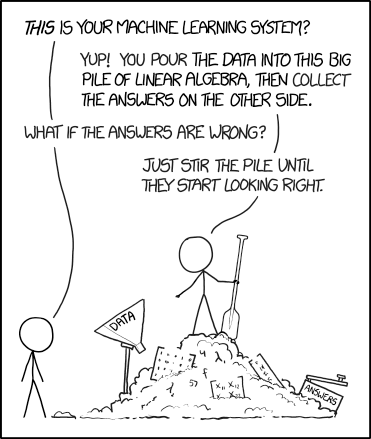
\includegraphics[width=\textwidth]{images/placeholder.png}
    \caption{Beispiele der Vorhersagen des Convolutional Neural Network. %
    Aufgezeigt ist zu einem Satellitenbild die Maske aus dem Datensatz und %
    die vorhergesagte Maske mit und ohne binärisierung über den Schwellwert. %
    Außerdem sind die zugehörigen Länder aufgelistet.}
    \label{fig:beispiele_cnn}
\end{figure}

\begin{figure}
    \centering
    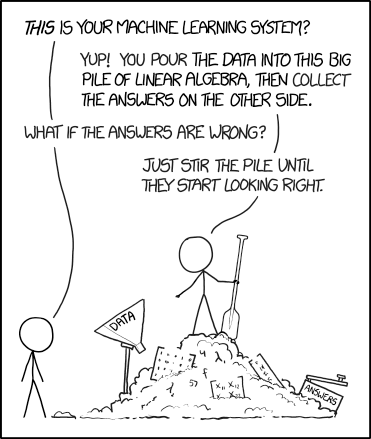
\includegraphics[width=\textwidth]{images/placeholder.png}
    \caption{Beispiele der Vorhersagen des Random Forest. %
    Aufgezeigt ist zu einem Satellitenbild das Bild der Gradienten, %
    die Maske aus dem Datensatz und %
    die vorhergesagte Maske mit binärisierung über den Schwellwert. %
    Außerdem sind die zugehörigen Länder aufgelistet.}
    \label{fig:beispiele_rndf}
\end{figure}

Es ist zu erkennen, dass die Ergebnisse teilweise besser sind als die gegebene Maske.
%%
%% Ergebnisse beschreiben
%%

Im Vergleich der Alternativmethode mit der Hauptmethode ist deutlich zu erkennen, 
dass die Alternativmethode pixelweise stattgefunden hat und die Vorhersagen haben ein gewisses Rauschen.
%%
%% Alternativ Ergebnisse beschreiben
%%

